\chapter{Results}
\section{\label{section:the_data}The AOLME Dataset}
The AOLME dataset is an enormous repository of over 900 hours of video
recordings of students [reference needed]. The videos contain students
interacting with facilitators, their peers and computers to write code in
Python on the Raspberry Pi.  The dataset is wealth of information but difficult
to exploit in its current state.  The data used for this thesis is a subset of
the entire AOLME dataset. By hand, we have selected several videos and extracted
typing and writing clips from the original dataset and are using these as ground
truth for measuring the accuracy of our classification. Figure \ref{fig:typing_writing}
is representative of the features that have been extracted by hand.

\begin{figure}[h]
  \label{fig:typing_writing}
  \centering
  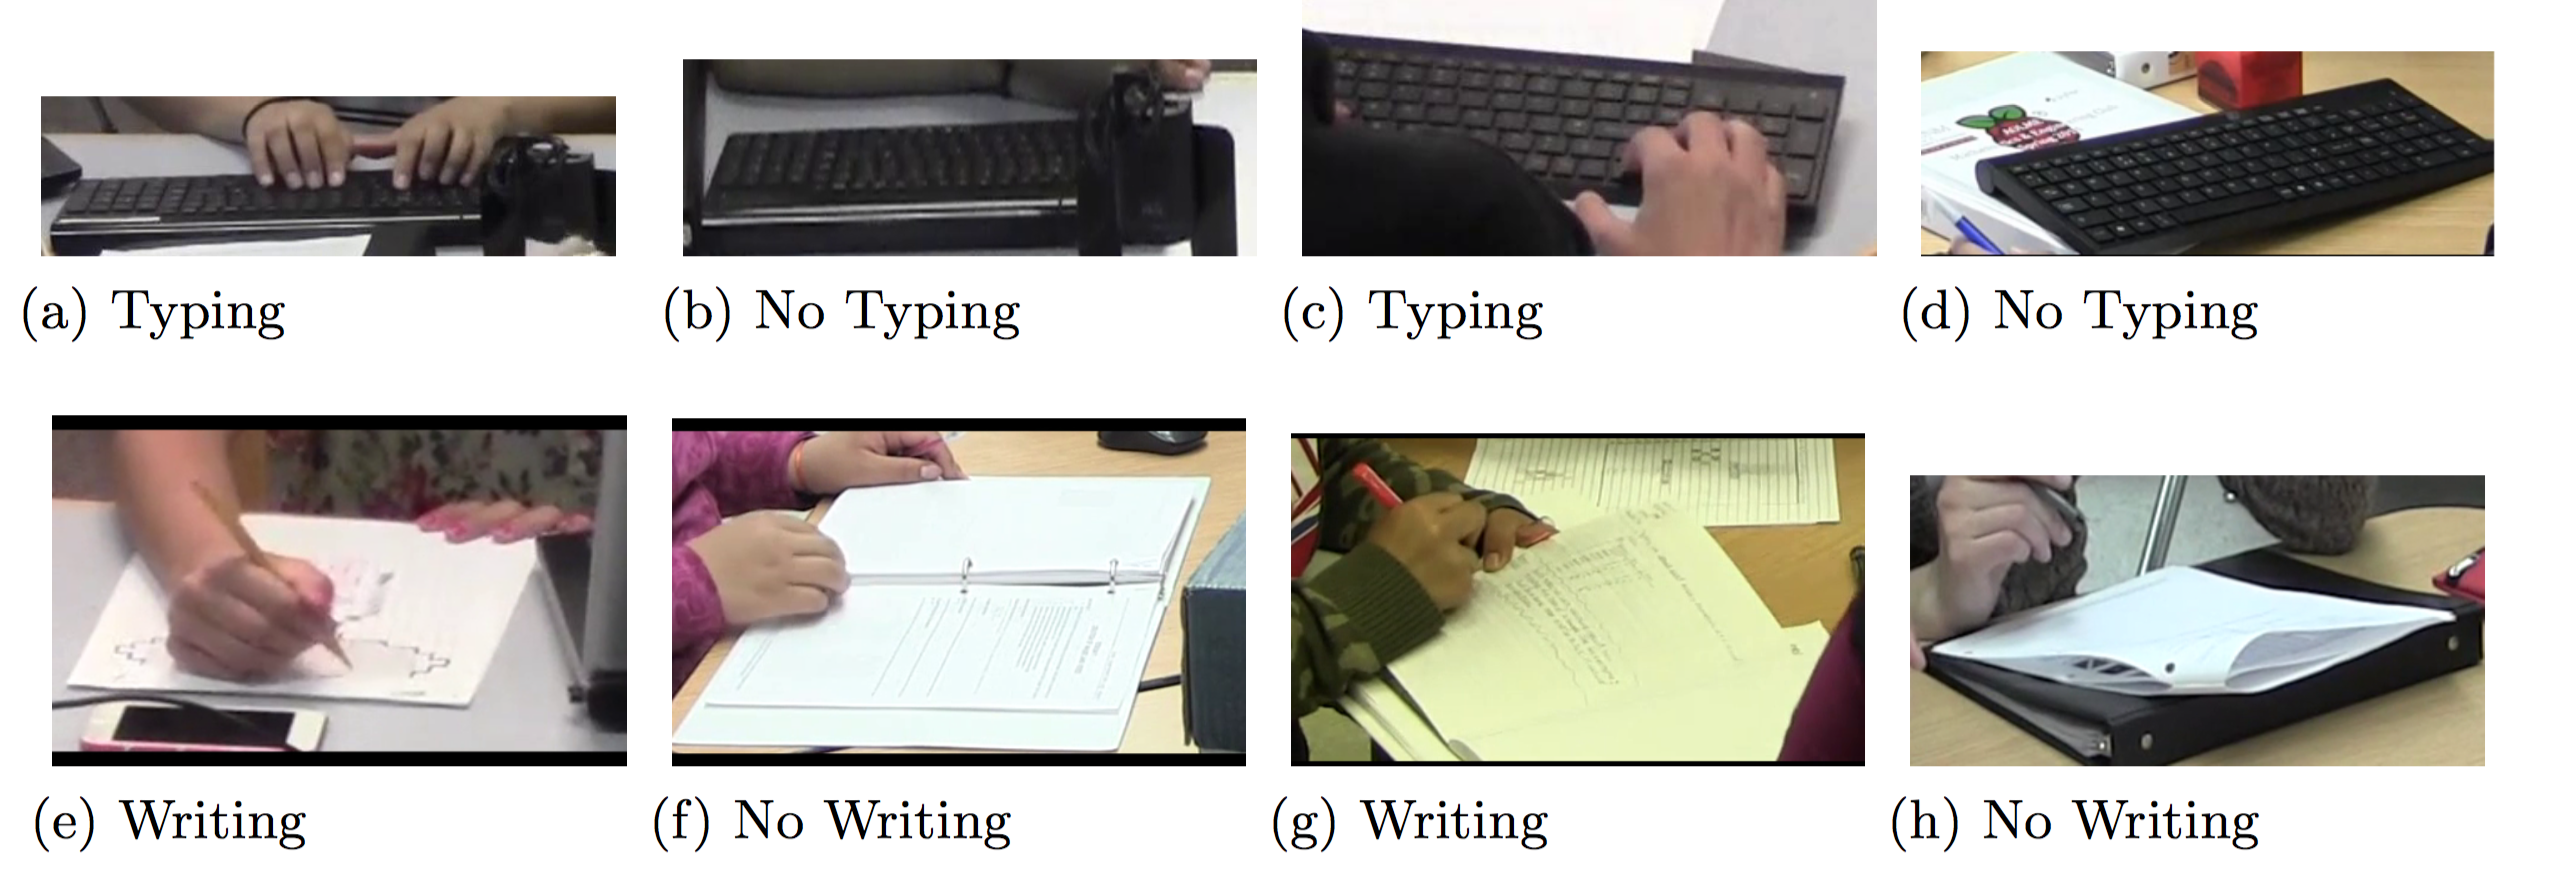
\includegraphics[width=\textwidth]{figures/typing_writing_clip}
  \caption{Example of features that have been manually extracted from the dataset
  for training and testing. For the above example, we need to classifiers for each
  activity to determine if the activity is being performed, or it is not.}
\end{figure}

As Figure \ref{fig:typing_writing} suggests, we are only using a cropped version
of the video. The reason for this is that we are not attempting to solve the tracking
problem in this thesis, only the classification problem. Hence, we assume that
the videos entering into our software have already been clipped and cropped with
the target activities inside of them and the corresponding lack of the activity.
Our subset of the AOLME database consists of the following:

\begin{itemize}
\item Twenty videos of typing
\item Twenty videos of no typing
\item Twenty videos of writing
\item Twenty Videos of no writing
\end{itemize}
